\documentclass{article}

\pagestyle{myheadings}

\usepackage{graphicx}
\usepackage{amsmath}
\usepackage{cite}
\usepackage{tikz}
\usepackage{verbatim}
\usepackage{verbatim}
\usepackage[active,tightpage]{preview}
\usepackage{fancyheadings}

\pagestyle{fancy}

\fancyhead[C]{Team 53506}
\fancyhead[R]{\thepage}

\usetikzlibrary{arrows}

\title{Safer Migration Strategies For Refugee Populations}
\author{Team 53506}

\begin{document}

\pagenumbering{gobble}
\maketitle
\tableofcontents

\maketitle

\newpage

\pagenumbering{arabic}

Humanitarian organizations that aim to settle refugees in Europe are currently facing new challenges because refugees are coming from outside Europe in larger numbers than ever before \cite{simpson}. One of these organizations, the office of the United Nations High Commissioner for Refugees (UNHCR) was initially formed in 1950 with the intent to help Europeans displaced by World War II \cite{historyUNHCR}. Since its inception the UNHCR has provided aid to refugees, internally dispaced people, stateless people, and asylum seekers from emergencies originating within Europe and, increasingly, outside of Europe \cite{historyUNHCR}.

Conflict and poor governance are seen as the main reasons that people become refugees \cite{simpson}. The 1951 refugee convention defines a refugee as ``owing to a well-founded fear of being persecuted for reasons of race, religion, nationality, membership of a particular social group or political opinion, is outside the country of his nationality, and is unable to, or owing to such fear, is unwilling to avail himself of the protection of that country'' \cite{1951convention}, rather than a migrant, who is someone moving from one country to another without refugee status. According to data from the UNCHCR Global Trends 2014, ongoing conflicts in Syria and Afghanistan are the largest source of refugees \cite{refugeefactsheet}. For our purposes refugees and migrants will be treated equivalently, because immigrants entering Europe are often lacking official refugee status before reaching their destination so it can be impossible to distinguish from a data set whether a migrant will be classified as a refugee or an economic migrant. When considering how to solve the refugee crisis, it is important to pair dealing with the root causes with safe and efficient relocation of refugees.

Any proposal regarding large volumes of refugee movement should be considered a short term proposal. The resources available for refugee aid are finite, and the impetus for humanitarian aid may decrease over time, causing assumptions that are used to determine optimal travel routes to become inaccurate over longer time periods. The only way to permanantly ease the migrant situation in Europe is to end the conflicts that make people flee their countries in the first place. Therefore, we should only project our models into short time periods in the future.

Immigrants travel multiple routes -- beginning at the middle east, and travelling through the West, East, and Central Mediterranean, the West Balkans, the Eastern Borders, and from Albania to Greece.
CITE TRAVEL MAP

\begin{center}
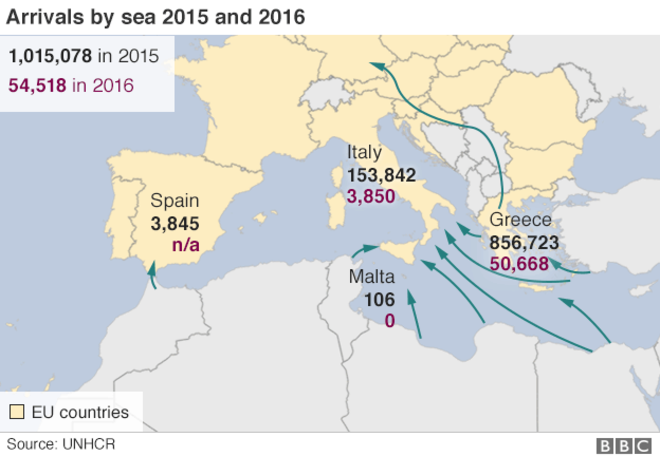
\includegraphics[scale=0.5]{travelmap}
\cite{BBCgraphics}
\end{center}

The political climate surrounding refugee aid in Europe is highly variable and subject to rapid change. Poorly managed camps in Hungary have damaged the reputation of migrants, leading to a surge in the popularity of the radical nationalist Jobbik party \cite{thorpe}. The way countries will handle immigration crises cannot be deterministically modeled, so this is considered to be an exogenous factor. In other countries, such as Germany, strong moral foundations protect the influx of immigration, with little (and strongly opposed) backlash at the new immigration policies \cite{hill}. In addition, unpredicted disasters such as the Paris attacks may threaten refugee relations with their host countries. In November 2015, the incoming Polish Minister for European Affairs said ``we will accept refugees only if we have security guarantees'' \cite{hewitt}. The Paris attacks deepened the level of mistrust towards refugees across Europe, since it was believed that the terrorists snuck into the country with refugees. Regardless of the truth of these facts (the only known attackers are French and Belgian residents), the coinciding events were treated as such, and has lead to border problems in the country. Although the only known terrorists were French and Belgian residents, if there is increased mistrust towards refugees that may lead to changes in publically acceptable refugee policy.

We have been tasked with building a model that will help develop a better understanding of the factors involved with facilitating the movement of refugees from their countries of origin into safe haven countries. In doing this, we are attempting to determine the safest and most efficient routes that refugees should take and how many refugees should travel along those routes at a time. The numbers of refugees that should take any given route will relate to the capacity of possible destinations within Europe and the number of refugees within the system. 


This problem breaks down into multiple problems.

\begin{enumerate}
    \item {\bf What are the factors involved with moving refugees?}

    The UN asks us to prioritize the health and safety of refugees. What attributes enable or inhibit the safe and efficient movement of refugees? The total number of refugees entering the system and at each node and the capacity of European countries to recieve countries are important variables within the system. The entry points for refugees, possible routes, the popularity and capacity of those routes, the length of routes, mode of transportation and availabilty of infrastructure for accomodation along those routes are parameters to be considered in the system.

    Safety will be optimized by minimizing the risk that any individual may not complete a route. We define a measure of risk that incorporates information about liklihood of illness, death (i.e. drowning on water routes), and other dangers of travel that may be exacerbated for routes with high throughput for a given route. We assume that low densities have low risk and that high densities have high risk. In the absence of data describing this relationship further, for simplicity we assume that population density on a route has a positive linear relationship to risk. If more data becomes available, then a more realistic density-risk function may be substituted into the model.

    To assess the efficiency of a route, one may consider a case with high numbers of migrants to determine where bottlenecks occur and the factors that are slowing down flow at that point on the graph. Efficiency can be incorporated into the selection of an optimal route by favouring shorter routes or including a penalty for slower travel and for long waits in camps before reaching the end destination and exiting the system. Policy that prevents a high number of individuals existing for long periods of time without settling in a country should be preferred.

    Assumptions: All migrants who make it to their destination travel at the average rate. Due to our choice of a linear programming model, all relationships are linear. Refugees are the only travellers along designated routes.

    \item {\bf How do we gain a better understanding of the factors?}

    It should be noted that in our system we must account for dynamically changing environmental factors. Our model should exhibit an allocation of resources in responce to endogenous changef to form the best route planning approach. Exogenous parameters (unavoidable, unpredictable events, like the terrorist attack in France) must also be considered.

    To gain a better understanding of the factors involved in refugee movement we will create a model of optimal refugee movement, considering accessibility of transport, safety of route, and resource capacities of countries. 

    We consider European and select neighbouring countries as nodes on a graph. Edges represent the paths on which refugees may travel. If policy is implemented so that refugee travel to and from a specific country is blocked, then the connectivity of that point is set to zero to represent an absence of refugee travel to that country. Given a known number of refugees at a number of entry points. Need to optimize distribution.

    Modelling methods considered:
    Stochastic Differential Equations are used in the stock market because individual factors cannot be influenced. This may be a way to realistically model the randomness of individual refugee movement. However, this type of model is difficult to optimize, which may make it difficult to meet our objective to optimize refugee movement. The use of stochastic programming may allow for optimization of the model. Stochastic effects are generally more important when you are dealing with small population sizes \cite{vries}. Since stochastic effects will likely have little impact on the overall movement of large groups of refugees along major migration routes, it is reasonable to model this situation using deterministic models for an initial model of the system.

    Modelling refugee movement may be treated as a social network problem, with multiple sources and sinks. Travel through the system may be described using fluid dynamics with partial differential equations describing each time step. 

    What do we know about our system?
    How much feedback exists in our system? Is it a closed system? 
    Let us consider a model that describes refugees that are not settled. This includes migrants who are residing in refugee camps in the Middle East, migrants who are in transit, and migrants who have reached a destination, but do not have accepted migrant status and have not been officially settled in the country. If a migrant becomes officialty settled then they have left the system. 

    Starting with a basic model, each possible country near Europe where there may be a substantial refugee population is represented as a vertex on a graph. The edges between vertices represent the connectivity between locations for refugees. Rates of travel along edges may vary based on qualities of the travel route including capacity, distance, modes of transportation available and risk to migrants. Once these variables and parameters are related on a graph, we need to learn about the dynamics of the system.

    One way to inform the movement of refugees from their country of origin into safe haven countries is to learn about how our system behaves when safety and efficiency are optimized. Safety and efficiency are optimized when risk and route length are minimized, respectively. Risk and length can be combined linearly, resulting in an overall measure that determines We chose to use linear programming (as in \cite{bertsekas}) to optimize our system because it can always be solved. 

\section{Refugee Movement Optimization}

Our goal is to identify optimal travel routes for refugees seeking asylum. Ongoing conflicts in Syria, Afghanistan, the Middle East, and Africa are critical contributors \cite{refugeefactsheet}. Data shows most of these refugees flee to neighboring Middle Eastern countries, and on to Europe \cite{refugeefactsheet}. Our investigation focuses on these groups, and their transportation to the most popular states. To guide transportation, we optimize a refugee transportation model, from the conflicts discussed to the Middle East and Europe. Economically, it is not feasible to transport large numbers of refugees by plane or boat, so we will not address refugee movement in this model.

We consider an optimization problem under realistic constraints to find the safest and most efficient solution for numbers of refugees on each route achievable. Most optimization problem are not computationally feasible. Therefore, we restrict our model to linear and quadratic programming methods. Each route will be associated with an allocation of refugees. The UNs primary goal in this matter is to safeguard the well-being of refugees during the journey \cite{UNStatement}. Such safety concerns will be incorporated into our model as a risk parameter, which we attempt to minimize. Factors such as overcrowding, route danger, and route length will contribute most to this risk. Sometimes, it may be worth a risky journey to end up in a country which is least risky to live in.

Recommended refugee quotas for each country based on the GDP and population of that country will enable us to approximate the refugee capacity of each country we are considering. By additional analysis of refugee statistics, we can estimate the projected refugees produced in 2016. Details of these described statistics require further analysis of available data than we were able to achieve in the course of the competetion.

Our model assumes the use of such statistics, provided as a parameter for the system. We shall denote the capacity of a country $w$ as $C_w$, and the refugee productions of a country $v$ as $R_v$. The model detailed assumes that $\sum R_v \leq \sum C_w$, to obtain a feasible solution to the optimization procedure. Of course, as we can see from the European reaction to the refugee crisis, there may be a much greater demand of resources than can be accomodated. Regardless of a country's refusal to admit more refugees, desparate refugees will find a way to flee their home country, though perhaps to a subacceptable destination. To model this, we place `substandard' camps with capacities large enough to contain what other countries are unable to maintain.

We begin by forming a directed graph, whose nodes are countries, and whose edges are possible paths for refugees to take to obtain asylum. We consider any particular refugee's journey to be a simple path in the graph, because refugees are unlikely to take cyclic routes. More importantly to us, the UN should not guide refugees to take such non-optimal routes. For each simple path $(v_1, \dots, v_n)$, we allocate a number $x_{(v_1, \dots, v_n)} \in \mathbf{R}$, which represents the approximate number of refugees travelling along that path. The constraints are summarized by the equations below.

\begin{enumerate}
    \item (No Refugee Left Behind) For every country $v$ producing refugees,
    %
    \[ \sum_{\substack{(v_1, \dots, v_n) \\ v_1 = v}} x_{(v_1, \dots, v_n)} = R_v \]
    %
    Where $R_v$ is the number of refugees exiting the country $v$.

    \item (Bounded Capacity) For each asylum country $w$,
    %
    \[ \sum_{\substack{(v_1, \dots, v_n) \\ v_n = w}} x_{(v_1, \dots, v_n)} \leq C_w \]
    %
    Where $C_w$ is the capacity of the country $w$.
\end{enumerate}

We formulate risk as a quadratic functional, with certain quantified factors described below.

\begin{enumerate}
    \item {\it The risk of a route}. Each edge $(v,w)$ in the graph is associated with a certain `risk constant' $K_{(v,w)}$ that represents the probability of death for a single refugee travelling along that edge. If $n$ refugees travel along this path, then the expected number of deaths will be $n K_{(v,w)}$. The risk of death travelling along a certain path $(v_1, \dots, v_n)$ is then compounded. By basic laws of probability, we have
    %
    \[ \mathbf{P}(\text{immigrant dies on}\ (v_1, \dots, v_n)) = \sum_{i = 1}^{n-1} \mathbf{P}(\text{immigrant dies on}\ (v_i, v_{i+1})) \]
    %
    We obtains an analogous equation for the risk constant, where the chance an immigrant dies on an edge is the product of the probability that the immigrant does not die on all previous edges, compounded with the probability that the immigrant dies on the final edge.
    %
    \[ K_{(v_1, \dots, v_n)} = \sum_{i = 1}^n \left( \prod_{j = 1}^{i-1} \left(1 - K_{(v_j,v_{j+1})} \right) \right) K_{(v_i, v_{i+1})} \]

    \item {\it Route overcrowding}. In an overcrowded group of refugees, disease, violence, and crime are likely to cause harm, so we must manage traveller density in order to reduce risk. We assume the number of interactions within a population is quadratically proportional to population density. It follows that the risk factors of disease, violence and crime, all due to population interaction, are also quadratically propertional to density. We assume that there exists a constant $B_{(v_1, \dots, v_n)}$ for each route $(v_1, \dots, v_n)$ such that the health compromising rates for a group of $n$ people are proportions to $B_{(v_1, \dots, v_n)} n^2$. We shall also have to consider `correlation rates', since two paths $(v_1, \dots, v_n)$ may coincide in such a way to cause congestion, leading to a rate of the form $B_{(v_1, \dots, v_n), (w_1, \dots, w_m)} n m$, where $m$ is the group travelling along a path $(w_1, \dots, w_m)$. Of course, for routes that never coincide, this value may be zero. For notational homogeneity, we shall also denote $B_{(v_1, \dots, v_n)}$ by $B_{(v_1, \dots, v_n), (v_1, \dots, v_n)}$. Derivation of these constants will be obtained in the next section.
\end{enumerate}

Our risk functional and constraints form a quadratic program. To summarize, our quadratic program is described in the following form.
%
\begin{align*}
    &\text{min} \sum_{(v_1, \dots, v_n)} K_{(v_1, \dots, v_n)} x_{(v_1, \dots, v_n)}\\
    & \ + \sum_{\substack{(v_1, \dots, v_n)\\(w_1, \dots, w_m)}} B_{(v_1, \dots, v_n) (w_1, \dots, w_m)} x_{(v_1, \dots, v_n)} x_{(w_1, \dots, w_m)}\\
    &\text{s.t. for each source $v$ and sink $w$,}\\
    &\ \ \ \ \ \sum_{\substack{(v_1, \dots, v_n) \\ v_1 = v}} x_{(v_1, \dots, v_n)} = R_v\\
    &\ \ \ \ \ \sum_{\substack{(v_1, \dots, v_n) \\ v_n = w}} x_{(v_1, \dots, v_n)} \leq C_w
\end{align*}
%
Any of your favourite quadratic optimization methods will find an optimum solutions to this problem.

\section{Deriving Path Correlation Coefficients}

In its current form, our linear program does not take into account the intersection of paths formed by travelling refugees. It also assumes that groups of refugees travel deterministically. This obviously does not hold in any practical sense -- No two refugees are completely alike, and react differently in response to different events.

Intersection of different refugee paths becomes an issue when trying to find the path correlation coefficients $B_{(v_1, \dots, v_n) (w_1, \dots, w_m)}$. Consider the diagram below, consisting of two curves, together with parameterizations $c$ and $c'$ with unit velocity. These curve represent one of the possible paths that refugees can take. When we model the movement of refugees as a single point on the line, then the movement of two groups of refugees coincides when $c(t) = c'(t)$. If the traces of $c$ and $c'$ intersect, but hit all points in the intersection at different times, then our model would determine that these groups never meet each other. On the other hand, we cannot just take the traces as evidence for congestion, for we would like to increase the importance of an intersection $c(t) = c(t')$ when $t$ and $t'$ are very close, and decrease the importance when the time points are far apart. After a long time, most refugees will have moved away from this point, so congestion is near negligable. We solve this problem by taking a stochastic movement along these curves, determining the expected intersection probability when two groups encounter one another.

\begin{center}

\end{center}

To accomodate the random motion of population migration, we apply the theory of stochastic processes, as developed in \cite{lawler}. Begin by making the following assumptions
%
\begin{enumerate}
    \item {\it Every immigrant starts the route at the start point.} Technically, immigrants could leave from various parts of a certain country, or join a group of refugees after they have already begun travelling.
    \item {\it The movement of immigrants, as a function of time, is continuous}. Physically, this assumption should always be satisfied.
    \item {\it The process of immigration movement is Markovian.} Past movement of a certain immigrant cannot predict future movement of that immigrant, aside from where the immigrant is at a certain timepoint. This assumption is to obtain a feasible solution. Though for a specific immigrant this assumption will not be satisfied, when we take statistical averages of immigration this assumption should at least be a good approximation.
    \item {\it Immigrant travel spreads according to a normal distribution}. This represents a `diffusion' of immigrants over time as they travel to their destination, which converges to the final destination asymptotically. By the law of large numbers, the distribution of immigrants should be sufficiently approximated by a normal distribution, so this assumption is not too sensitive to change.
\end{enumerate}
%
Now we calculate the coefficient of immigration. First, we pull back the curve $c$ to its domain $[0,A]$, and extending the definition of $c$ to $\mathbf{R}$, by definining $c(A + t) = c(A)$, $c(-t) = 0$ for $t \geq 0$. We shall place a stochastic process on the interval. The assumptions above uniquely determine the structure of the process. Since $c$ has unit velocity at all time points, we can describe the process $X_t$ which models the movement of immigrants via the stochastic equation
%
\[ X_t = \varepsilon W_t + t \]
%
where $\varepsilon$ is a small constant, and $W_t$ is standard brownian motion. We construct an independant task for each path $(v_1, \dots, v_n)$, represented by a curve $c$. If $X_t$ is such an equation, then $c(X_t)$ gives us a stochastic process on the path in the graph. We wish to measure, in some capacity, the `population correlation' between the stochastic processes $c(X_t)$ and $c'(Y_t)$. We cannot use the probability that two particular instances of the motion meet at a certain time point, since $\mathbf{P}(c(X_t) = c'(Y_t)) = 0$ for all values of $t$. The best we can do is approximate two populations coinciding; fixing a small $\varepsilon'$, we consider the `intersection measure'
%
\[ B_{(v_1, \dots, v_n), (w_1, \dots, w_m)} = \int_0^\infty \int_0^1 \mathbf{P}\left(c'(Y_t) - \varepsilon' < c(X_t) < c'(Y_t) + \varepsilon'\right)\ dY_t\ dt \]
%
which sums up the possible instances of intersection. Theoretically, this is an approximation. Practically, this method should perform well in practice; really, two people can never be in the {\it exact} same location at a particular time, so our model really does model the correct situation, provided we pick $\varepsilon'$ so that `vicinity' is small enough for two populations to affect one another, and big enough to obtain accurate interaction estimates. To calculate the integral, we perform some method of approximation. Due to the arbitrary nature of the parameterizations, an analytic form is impossible to obtain.

Our method above also allows us to extend our model to additional timeframes. We can now consider waves of immigrants, which begin at different time periods. Using the correlation coefficient determination method above (modified to take into account different time parameterizations).

\section{Metrics of Refugee Crisis}

\begin{center}
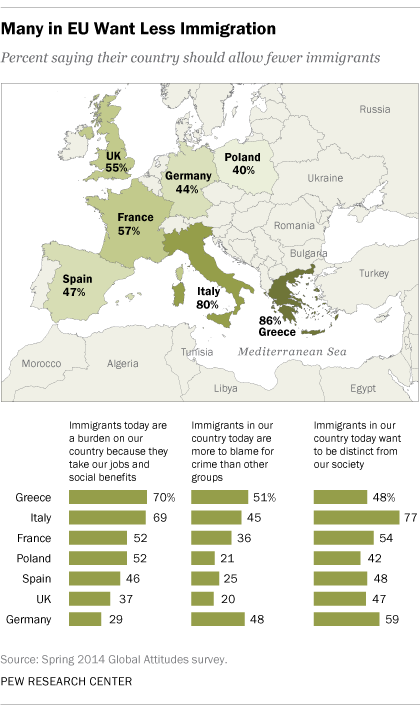
\includegraphics[scale=0.5]{ImmigrationPoll}
\end{center}

\bibliographystyle{plain}
\bibliography{refugee_citations}

\end{document}